\documentclass[12pt,a4paper,listof=totocnumbered, bibliography=totocnumbered,oneside]{scrbook}

\usepackage[ngerman]{babel} 						%Deutsche Trennung
\usepackage[utf8]{inputenc}						    %Zeichensatz
%\usepackage[numbers]{natbib}					    %Zusätzliche Simbole

\usepackage[backend=biber]{biblatex} 
\bibliography{Literatur}
	
\usepackage{amsmath}        					    %MathePacket
\usepackage{amsfonts}						        %Zusätliche Mathezeichen
\usepackage{amssymb}							    %Zusätzliche Mathezeichen wie Pfeile 
\usepackage[]{graphicx}					            %Packet für Bilder

\usepackage[headsepline,footsepline,plainfootsepline,markcase=upper]{scrlayer-scrpage}
\usepackage{tabularx}							    %Tabellen
\usepackage{tabu}
\usepackage{geometry}							    %Seitengeometrie
\usepackage[onehalfspacing]{setspace}			    %Zeilenabstand
\usepackage[printonlyused]{acronym}			    %Abkürzungen
\usepackage{subfig}								    %mehrere Bilde
%\usepackage{floatflt}							    %Objekte von Text umfließen lassen
\usepackage{float}								    %Positionierung von Objeten
\usepackage{wrapfig}							    %Objekte von Text umfließen lassen
\usepackage[usenames,dvipsnames]{color}		    %Farben für Latex
\usepackage{colortbl}							    %Farben für Tabellen
\usepackage{paralist}							    %Auflistungen
\usepackage{array}							        %Tabllen und mAtrizen in Matheumgebung
\usepackage{titlesec}							    %Überschriften verändern
\usepackage{parskip}							    %Absätze einstellen
%\usepackage{picins}							    %Umfließen vom Text
\usepackage[subfigure,titles]{tocloft}			    %Inhaltsverzeichnis formatieren
\usepackage[breaklinks=true,pdfpagelabels=true]{hyperref}%Verlinkungen erstellen
\usepackage{listings}							    %Quellcode einfügen
\usepackage{siunitx}							    %SI Schreibweise
\usepackage{chngcntr}							    %figurennumerierung
\usepackage[hyphenbreaks]{breakurl}			    %Zeilenumbruch links
%\usepackage{multibib}							    %mehrere literaturverzeichnisse
%\usepackage{times}								    %Times new roman
\usepackage{longtable}							    %Tabellen über mehrere Seiten
\usepackage{framed}								    %Rahmen
\usepackage{diagbox}							    %Diagonalboxen für Tabellen
\usepackage{xcolor}								    %noch mehr Farben						
\usepackage{nicefrac}							    %schöne Brüche
\usepackage{textpos}							    %Positionierung von Text
\usepackage{multicol}

\usepackage{booktabs}
\usepackage{pgfplots}
\usepackage{pgfplotstable}
\usepackage{tikz}
\usepgfplotslibrary{units}
%\pgfplotsset{compat=1.10}
\usepackage{caption}

%Eigene Farben
\definecolor{lightgray}{gray}{0.90}
\definecolor{tableheadergray}{gray}{0.95}
\definecolor{limegreen}{HTML}{E1F5A9}
\definecolor{tured}{HTML}{C50E1F}
\definecolor{tugrey}{HTML}{717171}

\newenvironment{cmssb}{\fontfamily{cmss}\fontseries{bx}\fontshape{n}\selectfont}{\par}
\newenvironment{cmss}{\fontfamily{cmss}\fontseries{m}\fontshape{n}\selectfont}{\par} 


%Geometrie der Seite Einrichten
\geometry{a4paper, top=20mm, left=25mm, right=15mm, bottom=20mm, headsep=5mm, footskip=10mm}
%\areaset{15cm}{20cm}

\lohead[]{}
\cohead[]{}
\rohead[]{}
\lehead[]{}
\cehead[]{}
\rehead[]{}
\lofoot[]{}
\cofoot[Seite \pagemark]{Seite \pagemark}
\rofoot[]{}
\lefoot[]{}
\cefoot[]{Seite \pagemark}
\refoot[]{}

%\ModifyLayer[addvoffset=-2pt]{scrheadings.foot.above.line}
\setkomafont{pagehead}{\normalfont\color{tugrey}}
\setkomafont{pagefoot}{\small\normalfont\color{tugrey}}
\setkomafont{headsepline}{\color{tugrey}}
\setkomafont{footsepline}{\color{tugrey}}

\makeatletter 
\renewcommand{\l@figure}{\@dottedtocline{1}{1.5em}{3em}} 
\renewcommand{\l@table}{\@dottedtocline{1}{1.5em}{3em}} 

%Nummerierungen
\numberwithin{figure}{chapter}			    %Nummerierung der figuren
\numberwithin{equation}{chapter}		        %Nummerierung der formeln

% Abstände Überschrift
\titlespacing{\section}{0pt}{12pt plus 4pt minus 2pt}{-6pt plus 2pt minus 2pt}
\titlespacing{\subsection}{0pt}{12pt plus 4pt minus 2pt}{-6pt plus 2pt minus 2pt}
\titlespacing{\subsubsection}{0pt}{12pt plus 4pt minus 2pt}{-6pt plus 2pt minus 2pt}

\pagenumbering{Roman}
\renewcommand\thechapter{\Roman{chapter}}
\renewcommand\thesection{\roman{section}}


%-------------------
\begin{document}
    \begin{titlepage}
    \newgeometry{left=24mm, right=8mm, top=10mm, bottom=13mm}
	\begin{textblock*}{0mm}(110mm,0mm)
			
\includegraphics[width=60mm]{Abbildungen/Deckblatt-Beuth/Beuth_Logo.png}  
	\end{textblock*} 

\vspace*{4cm}
    
    \begin{cmssb}
    	\begin{flushleft}
    		%\textcolor{tured}{\rule{13cm}{.4pt}}\\
    		\vspace*{10pt} 
    		\textsf{\fontsize{14}{0}\selectfont Beuth Hochschule für Technik Berlin  Fachgebiet Medieninformatik}\\
			\vspace*{10pt} 
			\textsf{\fontsize{30}{0}\selectfont Masterarbeit}\\
			\vspace*{10pt}
			\textcolor{tured}{\textsf{\fontsize{14}{0}\selectfont Cloud-basierte Datenerfassung und Visualisierung für Fahrzeugdaten.}}
			%\textcolor{tured}{\rule{13cm}{.4pt}}\\
		\end{flushleft}
	\end{cmssb}
 
\begin{textblock*}{60mm}(120mm,10mm)
    \begin{flushleft}
    	\begin{cmss}
    		\begin{normalsize}		
    			\textcolor{tugrey}{Vorgelegt von:}\\
				Jawhar Ben Hadj M'Barek\\
				Franz Mehring Platz. 3\\
				10243 Berlin \linebreak\linebreak
				Mat.-Nr. 837072\\
				s63338@beuth-hochschule.de
				\linebreak\linebreak\linebreak
				\textcolor{tugrey}{Erstprüfer:}\\
				Prof. Dr. Sven Graupner\\
				\textcolor{tugrey}{Zweitprüfer:}\\
				Prof. Dr. Siu\\
				\textcolor{tugrey}{Abgabe:}\\
				26. November 2018\linebreak\linebreak
			\end{normalsize}	
		\end{cmss}
    \end{flushleft}    
\end{textblock*} 	

\end{titlepage}

\newpage

\thispagestyle{empty}

    %\pagebreak
%leer
%\thispagestyle{empty}
%\pagebreak
\section*{Selbstständigkeitserklärung}
\vspace{5cm}
\begin{framed}
Hiermit erkläre ich, dass ich die vorliegende Arbeit selbstständig und eigenhändig sowie ohne unerlaubte
fremde Hilfe und ausschließlich unter Verwendung der aufgeführten Quellen und Hilfsmittel angefertigt habe.\\

Berlin, den\\

............................................................................................................\\
Unterschrift
\end{framed}
\newpage


    \setcounter{page}{2}
    \chapter{Zusammenfassung/Abstract}
    \section{Zusammenfassung}
        Text Text Text Text Text Text Text Text Text Text Text Text Text Text Text Text Text Text Text Text Text Text Text Text 
        Text Text Text Text Text Text Text Text Text Text Text Text Text Text Text Text Text Text Text Text Text Text Text Text
        Text Text Text Text Text Text Text Text Text Text Text Text Text Text Text Text Text Text Text Text Text Text Text Text
        Text Text Text Text Text Text Text Text Text Text Text Text Text Text Text Text Text Text Text Text Text Text Text Text
        Text Text Text Text Text Text Text Text Text Text Text Text Text Text Text Text Text Text Text Text Text Text Text Text
    \section{Abstract}
        Englischer Text Englischer Text Englischer Text Englischer Text Englischer Text Englischer Text Englischer Text Englischer Text             
        Englischer Text Englischer Text Englischer Text Englischer Text Englischer Text Englischer Text Englischer Text Englischer Text 
        Englischer Text Englischer Text Englischer Text Englischer Text Englischer Text Englischer Text Englischer Text Englischer Text 
        Englischer Text Englischer Text Englischer Text Englischer Text Englischer Text Englischer Text Englischer Text Englischer Text 
        Englischer Text Englischer Text Englischer Text Englischer Text Englischer Text Englischer Text Englischer Text Englischer Text 
    \tableofcontents
    %\lohead[]{llll}
\chapter{Nomenklatur}
    \section{Formelzeichen}
    \begin{longtable}[l]{p{3cm}|p{12cm}}
        Formelzeichen & Beschreibung\\
        \hline
        $A$ &Ausgabeschicht/Ruhelage\\
        $c$ & Koeffizienten im Polynom/Koeffizienten in Teststrecke \\
        $\vec{c}$ &Center-Vektor\\
        $\vec{d}$ & Abstand zwischen zwei Vektoren\\
        $E$ & Eingabeschicht/Fehler\\
        $e$ & Quadratischer Fehler\\
        $f$ & Funktion/Frequenz\\ 
        $flops$ & Fließkommaoperationen \\
        $g$ & Funktion/Parameter\\
        $H$ & Verborgene Schicht bzw. Layer\\
        $h$ & Funktion\\
        $I$ & Netzeingabe\\
        $|I|$ & Anzahl Beispiele\\
        $\vec{i}$ & Input eines einzelnen Neurons\\
        $J$ & Jacobimatrix\\
        $k$ & Anzahl \\
        $m$ & Anzahl der Ausgänge/ganzzahliges Vielfaches\\
        $N$ & Menge aller Neuronen\\
        $n$ & Anzahl Neuronen/Anzahl Trainingsbeispiele\\
        $O$ & Netzausgabe\\
        $o$ & Output eines einzelnen Neurons\\
        $P$ & Performance\\
        $p$ & Anzahl der Beispiele die erneuert werden\\
        $q$ & Grad des Polynoms/Anzahl der Layer\\
        $r$ & Zeitauflösung\\
        $s$ & Grenze bzw. Schranke\\
        $T$ & Ausgabemuster/Teachinginput\\
        $t$ & Zeit bzw. Zeitpunkt\\
        $u$ & Stellgröße\\
        $V$ & Menge aller Verbindungen\\
        $v$ & Gewicht/Polynom\\
        $W$ & Matrix aller Gewichte\\
        $\vec{w}$ & Eingangsgewichte eines einzelnen Neurons\\
        $w$ & Gewicht\\
        $Y$ & Messwert\\
        $y$ & Regelgröße\\
        $\vec{Z}$ & Innere Zustände eines Neurons\\
        &\\
        $\alpha$ & Parameter \\
        $\beta$ & Parameter \\
        $\Delta$ & Änderung \\
        $\delta$ & Gewichtsänderung\\
        $\eta$ & Lernrate\\
        $\Theta$ & Parameter\\
        $\mu$ & Regularisierungsfaktor\\
        $\rho$ & Korrelationswert\\ 
        $\tau$ & Integrationsvariable\\
        $\nabla$ & Nablaoperator \\
       
    \end{longtable}

    \section{Indizes}
    
    \begin{longtable}[l]{p{3cm}|p{12cm}}
        Index & Beschreibung\\
        \hline
        $A$ & Aktivierung\\
        $alt$ & alt/aus vergangenem Zeitschritt\\
        $i$ & Zählindex\\
        $j$ & Zählindex\\
        $k$ & Zählindex\\
        $last$ & Vergangene Werte\\
        $Modell$/$M$ & Größen die aus dem Modell berechnet wurden\\
        $max$ & Maximal\\
        $o$ & Ausgabe\\
        $P$ & Propagierung\\
        $p$ & Prediction\\
        $^p$ & Ein bestimmtes Trainingsmuster\\
        $q$ & Zählindex\\
        $rand$ & Zufällig\\  
        $s$ & Statisch\\
        $T$ & Teachinginput \\
        $Train$ & Training\\
        $Val$ & Validation\\            
        
        
    \end{longtable}

    \newpage
    %--------------Einstellungen Hauptteil--------------------
    \lohead[]{}
    \cohead[]{}
    \rohead[]{\headmark}
    \lehead[]{\headmark}
    \cehead[]{}
    \rehead[]{}
    \lofoot[]{}
    \cofoot[Seite \pagemark]{Seite \pagemark}
    \rofoot[]{}
    \lefoot[]{}
    \cefoot[]{Seite \pagemark}
    \refoot[]{}
    \pagenumbering{arabic}
    \setcounter{page}{1}
    \setcounter{chapter}{0}
    \renewcommand\thechapter{\arabic{chapter}}
    \renewcommand\thesection{\thechapter.\arabic{section}}
    %-------------Hauptteil------------------------------------
    \chapter{Einleitung}
    Einleitung Einleitung Einleitung Einleitung Einleitung Einleitung Einleitung Einleitung
    \section{Zielsetzung}
    Einleitung Einleitung Einleitung Einleitung Einleitung Einleitung Einleitung Einleitung

    
    
    \chapter{Technische Grundlagen}
    Text Text Text Text Text Text Text Text Text Text Text Text Text Text Text Text Text Text Text Text Text Text Text Text 
    Text Text Text Text Text Text Text Text Text Text Text Text Text Text Text Text Text Text Text Text Text Text Text Text
    Text Text Text Text Text Text Text Text Text Text Text Text Text Text Text Text Text Text Text Text Text Text Text Text
    Text Text Text Text Text Text Text Text Text Text Text Text Text Text Text Text Text Text Text Text Text Text Text Text
    \section{Messdaten Extraktion}
        Eine Section
        \subsection{CAN BUS und PEAK}
        \subsection{OBD und UDS Schnittetellen}
        
    \section{Übertragung in Cloud}
		\subsection{IOT und MQTT}
        Eine Subsection
		\subsection{AWS IOT und SDK}
        Eine Subsection
		\subsection{AWS Lambda Funktionen}
        Eine Subsection
		\subsection{AWS API Gateway}
        Eine Subsection
		und noch eine neue Seite
        \newpage
	\section{Datenablage und Visualisierung}
		\subsection{Elasticsearch}
        
		\subsection{DynamoDB}
        Eine Subsection
		\subsection{Kibana}
        Eine Subsection
		\subsection{JavaFx}
        Eine Subsection
        \newpage
	\section{Sprachsteurung}
        \subsection{AWS Alexa}
        Eine Subsection
		\subsection{AWS SNS}
        Eine Subsection
        \newpage
    \chapter{Lösungsansätze}
    Hier ein anderes Kapitel
    Viele Zitate: \cite{patterson} \cite{krizhevsky} \cite{matlab} \cite{pitts} \cite{lawrence} \cite{miesbach}
    \section{Elasticsearch vs. DynamoDB}
        
        The most important thing about Elasticsearch is that Elasticsearch supports full text search and that makes it different froms the normal databases, which are very much black and white, we just store stuff and retrieve it. In Full text search we look more for the concept, not a specific word in singular or in plural but we are looking for the concept or the meaning, which is very complicated to achieve with the normal databases for many reasons: building complicated queries, much more computing time by searching, long time for getting the response and by returning the result and not very performant like with Elasticsearch.
        
        Common Databases are focusing on how to store the data comparing to Elasticsearch that allows us to make sense of our data, explore them and be able to ask questions on the data in a simple way without writing complicated Query.
        Elasticsearch give us the ability to make data exploration, to go ahead and ask questions on the saved data and get results in milliseconds and be ready to visulise and make analytics on them.
               
        \subsection{Subsection}
            \begin{figure}[h]
                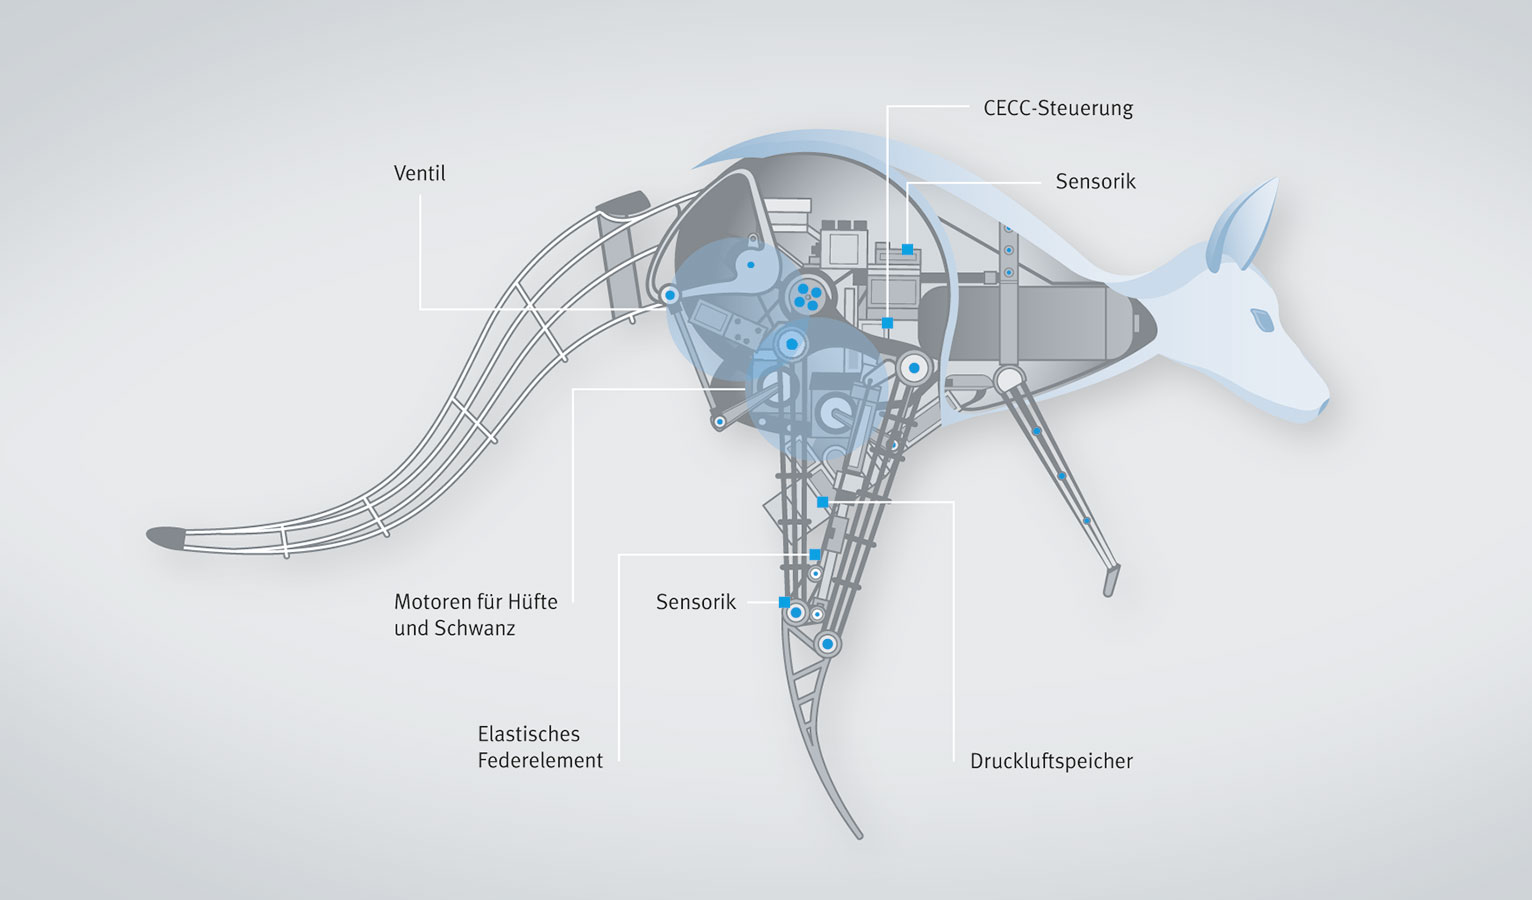
\includegraphics[scale=0.2]{Abbildungen/Kapitel2/Kangoroo.png}
                \centering
                \caption{Ein Kangoroo}
                \label{Abb:Kangoroo}   
            \end{figure}  
             \begin{table}[h]
                \begin{tabular}{ccc}
                      \hline
                      Spalte1 & Spalte2 & Spalte3\\                      
                      \hline
                      1 & 2 & 3\\
                      \hline
                \end{tabular}
                \centering
                \caption{Eine Tabelle}
                \label{Tab:Tabelle1}
            \end{table}
 
        
        
    \section{Kibana und JavaFx}
        Eine Subsection
        \newpage
        Eine neue Seite
        \newpage 
        Noch eine neue Seite
        \newpage    
        und noch eine neue Seite
    \chapter{Analyse}
    Hier ein neues Kapitel
    Viele Zitate: \autocite[]{patterson} \autocite[]{krizhevsky} \autocite[]{matlab} \cite{pitts} \cite{lawrence} \cite{miesbach}
    \section{Anforderungen}
        Eine Section
        \subsection{Echtzeitfähigkeit}
            \begin{figure}[h]
                \includegraphics[scale=0.2]{Abbildungen/Kapitel3/Big-architecture.png}
                \centering
                \caption{das Architekturbild}
                \label{Abb:Architekturbild}   
            \end{figure}  
             \begin{table}[h]
                \begin{tabular}{ccc}
                      \hline
                      Spalte1 & Spalte2 & Spalte3\\                      
                      \hline
                      1 & 2 & 3\\
                      \hline
                \end{tabular}
                \centering
                \caption{Variation über Zeit}
                \label{Tab:Tabelle3}
            \end{table}
            
Hier eine neue Tabelle   
            
            \begin{table}[h]
                \begin{tabular}{ccc}
                      \hline
                      Spalte1 & Spalte2 & Spalte3\\                      
                      \hline
                      1 & 2 & 3\\
                      \hline
                \end{tabular}
                \centering
                \caption{new added Tabelle}
                \label{Tab:New added}
            \end{table}
 
        
        
    \section{dynamische Erstellung von Diagramme}
        Eine Subsection
        \newpage
        Eine neue Seite
        \newpage 
        Noch eine neue Seite
        \newpage    
        und noch eine neue Seite
    \chapter{Design}
    Hier ein neues Kapitel
    Viele Zitate: \cite{patterson} \cite{krizhevsky} \cite{matlab} \cite{pitts} \cite{lawrence} \cite{miesbach}
    \section{Use Cases}
        Eine Section
        \subsection{Subsection}
        
        
Hier ist ein Bild:        
            \begin{figure}[h]
                \includegraphics[scale=0.2]{Abbildungen/Kapitel4/Big-architecture.png}
                \centering
                \caption{Affe Bild}
                \label{Abb:Affe}   
            \end{figure}  
            
Hier ist eine Tabelle: text text text text text text text text text text text text text text text text text text text text text text text text text text text text text text text text text text text text text text text text text text text text text text text text text text text text text text text text text text text text text text text text text text text text text text text text text text text text text text text text text text text text text text text text text text text text text text text text text text text text text text text text text text text text text text text text text text text text text text text text text.           
            
             \begin{table}[h]
                \begin{tabular}{ccc}
                      \hline
                      Spalte1 & Spalte2 & Spalte3\\                      
                      \hline
                      1 & 2 & 3\\
                      \hline
                \end{tabular}
                \centering
                \caption{Quadratewurzel Skalierung}
                \label{Tab:Quadratewurzel Skalierung}
            \end{table}
            
Hier eine neue Tabelle: text text text text text text text text text text text text text text text text text text text text text text text text text text text text text text text text text text text text text text text text text text text text text text text text text text text text text text text text text text text text text text text text text text text text text text text text text text text text text text text text text text text text text text text text text text text text text text text text text text text text text text text text text text text text text text text text text text text text text text text text text.   
            
            \begin{table}[h]
                \begin{tabular}{cccc}
                      \hline
                      Spalte1 & Spalte2 & Spalte3 & jbjvh\\                      
                      \hline
                      1 & 2 & 3 & 4\\
                      \hline
                \end{tabular}
                \centering
                \caption{Logaritmische Skalierung}
                \label{Tab:Logaritmische Skalierung}
            \end{table}
 
        
        
    \section{Modulendiagramm}
        Eine Subsection
	\section{Spezifikation von Datenstrukturen}
        Eine Subsection
	\section{Spezifikation von Schnittstellen}
        Eine Subsection
	\section{Klassendiagramm}
        Eine Subsection
  
    \chapter{Implementierung}
    Hier ein neues Kapitel
    Viele Zitate: \cite{patterson} \cite{krizhevsky} \cite{matlab} \cite{pitts} \cite{lawrence} \cite{miesbach}
    \section{Architektur}
        Eine Section
        \subsection{Subsection}
        
        
Hier ist ein Bild:        
            \begin{figure}[h]
                \includegraphics[scale=0.2]{Abbildungen/Kapitel4/Big-architecture.png}
                \centering
                \caption{Affe Bild}
                \label{Abb:Affe}   
            \end{figure}  
            
Hier ist eine Tabelle: text text text text text text text text text text text text text text text text text text text text text text text text text text text text text text text text text text text text text text text text text text text text text text text text text text text text text text text text text text text text text text text text text text text text text text text text text text text text text text text text text text text text text text text text text text text text text text text text text text text text text text text text text text text text text text text text text text text text text text text text text.           
            
             \begin{table}[h]
                \begin{tabular}{ccc}
                      \hline
                      Spalte1 & Spalte2 & Spalte3\\                      
                      \hline
                      1 & 2 & 3\\
                      \hline
                \end{tabular}
                \centering
                \caption{Quadratewurzel Skalierung}
                \label{Tab:Quadratewurzel Skalierung}
            \end{table}
            
Hier eine neue Tabelle: text text text text text text text text text text text text text text text text text text text text text text text text text text text text text text text text text text text text text text text text text text text text text text text text text text text text text text text text text text text text text text text text text text text text text text text text text text text text text text text text text text text text text text text text text text text text text text text text text text text text text text text text text text text text text text text text text text text text text text text text text.   
            
            \begin{table}[h]
                \begin{tabular}{cccc}
                      \hline
                      Spalte1 & Spalte2 & Spalte3 & jbjvh\\                      
                      \hline
                      1 & 2 & 3 & 4\\
                      \hline
                \end{tabular}
                \centering
                \caption{Logaritmische Skalierung}
                \label{Tab:Logaritmische Skalierung}
            \end{table}
 
        
        
    \section{Realisierungsspezifishe Probleme}
        Eine Subsection
	\section{Testkonzept und Testergebnisse}
        Eine Subsection
	\section{interessante Systemteile und Kode}
        Eine Subsection
    
    \chapter{Anwendung}
    Hier ein neues Kapitel
    Viele Zitate: \cite{patterson} \cite{krizhevsky} \cite{matlab} \cite{pitts} \cite{lawrence} \cite{miesbach}
    \section{System Bedienung}
        Eine Section
        \subsection{Subsection}
        
        
Hier ist ein Bild:        
            \begin{figure}[h]
                \includegraphics[scale=0.2]{Abbildungen/Kapitel4/Big-architecture.png}
                \centering
                \caption{Affe Bild}
                \label{Abb:Affe}   
            \end{figure}  
            
Hier ist eine Tabelle: text text text text text text text text text text text text text text text text text text text text text text text text text text text text text text text text text text text text text text text text text text text text text text text text text text text text text text text text text text text text text text text text text text text text text text text text text text text text text text text text text text text text text text text text text text text text text text text text text text text text text text text text text text text text text text text text text text text text text text text text text.           
            
             \begin{table}[h]
                \begin{tabular}{ccc}
                      \hline
                      Spalte1 & Spalte2 & Spalte3\\                      
                      \hline
                      1 & 2 & 3\\
                      \hline
                \end{tabular}
                \centering
                \caption{Quadratewurzel Skalierung}
                \label{Tab:Quadratewurzel Skalierung}
            \end{table}
            
Hier eine neue Tabelle: text text text text text text text text text text text text text text text text text text text text text text text text text text text text text text text text text text text text text text text text text text text text text text text text text text text text text text text text text text text text text text text text text text text text text text text text text text text text text text text text text text text text text text text text text text text text text text text text text text text text text text text text text text text text text text text text text text text text text text text text text.   
            
            \begin{table}[h]
                \begin{tabular}{cccc}
                      \hline
                      Spalte1 & Spalte2 & Spalte3 & jbjvh\\                      
                      \hline
                      1 & 2 & 3 & 4\\
                      \hline
                \end{tabular}
                \centering
                \caption{Logaritmische Skalierung}
                \label{Tab:Logaritmische Skalierung}
            \end{table}
 
        
        
    \section{gebliebene Fehlermeldungen und Ursachen}
        Eine Subsection
	\section{Nutzer Reaktion}
        Eine Subsection
  
    \chapter{Fazit}
    Hier schrieben wie gut alles war.

    %-------------Einstellungen Ende---------------------------
    %\pagenumbering{Roman}
    %\setcounter{page}{10}
    \setcounter{chapter}{2}
    \renewcommand\thechapter{\Roman{chapter}}
    \renewcommand\thesection{\roman{section}}
    %-------------Ende-----------------------------------------
	\printbibliography
%    \lohead[]{a}
%    \cohead[]{b}
%    \rohead[]{c}
%    \lehead[]{a2}
%    \cehead[]{b2}
%    \rehead[]{c2}
%    \lofoot[]{aa}
%    \cofoot[Seite \pagemark]{Seite \pagemark}
%    \rofoot[]{cc}
%    \lefoot[]{aa2}
%    \cefoot[]{bb2}
%    \refoot[]{cc2}
    
	\newpage
    \listoffigures
    \newpage
    \listoftables
    \chapter{Anhang}
    Das hier ist der Anhang
    \section{Section}
    \subsection{Subsection}

\end{document}
